\NeedsTeXFormat{LaTeX2e}
%\PassOptionsToClass{handout}{beamer}
\documentclass{beamer}
\usepackage{beamerPack}
\usepackage[boxed,ruled,vlined]{algorithm2e}
\usetikzlibrary{shapes.geometric,arrows,fit,matrix,positioning}
\tikzset{
  treenode/.style = {circle, draw=black, align=center, minimum size=1cm, anchor=center},
  subtree/.style = {regular polygon, regular polygon sides=3, draw=black, align=center, minimum height=0.8cm, minimum width=0.6cm, anchor=north}
}
\usepackage[03]{../lecture}
\subtitle{整列}
\begin{document}

\begin{frame}[fragile]{}
\titlepage
\end{frame}

\section{sort}		%%%%%%%%
\subsection{}

\begin{frame}[fragile]{整列}{}
\begin{itemize}\itemindent15mm\labelsep10mm
\item[初期状態]入力: 配列\texttt{VecT}

\medskip
\scalebox{0.6}{
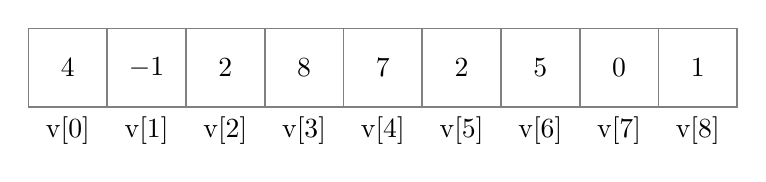
\begin{tikzpicture}[
    , cell/.style = {rectangle,draw=gray,semithick,minimum size=1cm,outer sep = 0mm,label=below:v{[\j]}}
]
\foreach \i [count=\j from 0] in {4, -1, 2, 8, 7, 2, 5, 0, 1}
    \node[cell] at (\j, 0) {$\i$};
\end{tikzpicture}
}
\item[最終状態]出力: 整列ずみの配列\texttt{VecT}

\medskip
\scalebox{0.6}{
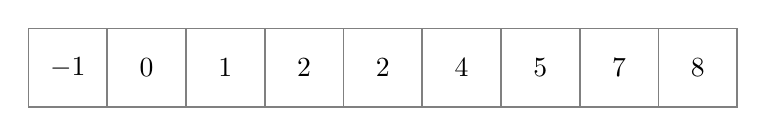
\begin{tikzpicture}[
    , cell/.style = {rectangle,draw=gray,semithick,minimum size=1cm,outer sep = 0mm}
]
\foreach \i [count=\j from 0] in {-1, 0, 1, 2, 2, 4, 5, 7, 8}
    \node[cell] at (\j, 0) {$\i$};
\end{tikzpicture}
}
\end{itemize}
全ての要素に順序がつけられること:全順序性が必要。
\vfill
\begin{block}{安定なソート}
順序が同じ要素は整列後も元の順序を保つ
\end{block}

氏名順に並んでいた学生データの配列を成績順にソート
\end{frame}

\section{bubble sort}		%%%%%%%%
\subsection{}

\begin{frame}[fragile]{バブルソート}{}
\scalebox{0.5}{
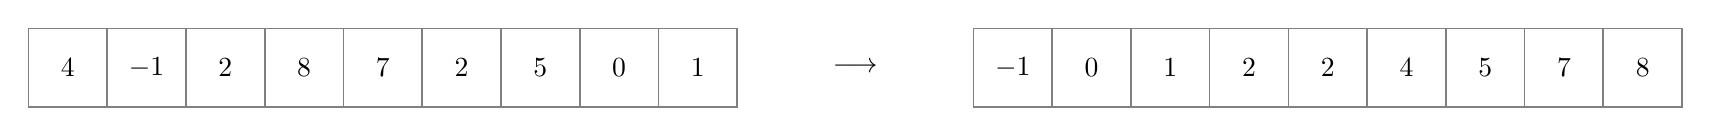
\begin{tikzpicture}[xshift=0.15\textwidth
    , cell/.style = {rectangle,draw=gray,semithick,minimum size=1cm,outer sep = 0mm}
]
\foreach \i [count=\j from 0] in {4, -1, 2, 8, 7, 2, 5, 0, 1}
    \node[cell] at (\j, 0) {$\i$};
\node at (10, 0) {$\longrightarrow$};
\foreach \i [count=\j from 0] in {-1, 0, 1, 2, 2, 4, 5, 7, 8}
    \node[cell] at (\j + 12, 0) {$\i$};
\end{tikzpicture}
}

\vfill
適切な中間目標を設定せよ

\vfill
先頭の1個が要件を満たしている

\vfill
\scalebox{0.6}{
\begin{tikzpicture}[cell/.style = {rectangle,draw=gray,semithick,minimum size=1cm,outer sep = 0mm}]
\foreach \i [count=\j from 0] in {-1, 0, 1, 2, 2, 4, 5, 7, 8}
    \node[cell] at (\j, 0) {$\i$};
\node[anchor=west] at (9,0) {中間目標になってない};
\end{tikzpicture}
}

\medskip
\scalebox{0.6}{
\begin{tikzpicture}[cell/.style = {rectangle,draw=gray,semithick,minimum size=1cm,outer sep = 0mm}]
\foreach \i [count=\j from 0] in {-1, 0, 0, 0, 0, 0, 0, 0, 0}
    \node[cell] at (\j, 0) {$\i$};
\node[anchor=west] at (9,0) {次のステップにいけない};
\end{tikzpicture}
}

\medskip
\scalebox{0.6}{
\begin{tikzpicture}[cell/.style = {rectangle,draw=gray,semithick,minimum size=1cm,outer sep = 0mm}]
\foreach \i [count=\j from 0] in {-1, 5, 2, 2, 8, 4, 0, 7, 1}
    \node[cell] at (\j, 0) {$\i$};
\node[anchor=west] at (9,0) {順番が変わってしまった。問題か?};
\end{tikzpicture}
}

\medskip
\scalebox{0.6}{
\begin{tikzpicture}[cell/.style = {rectangle,draw=gray,semithick,minimum size=1cm,outer sep = 0mm}]
\foreach \i [count=\j from 0] in {-1, X, X, X, X, X, X, X, X}
    \node[cell] at (\j, 0) {$\i$};
\node[anchor=west] at (9,0) {$X$は-1以外のもとからあった要素};
\end{tikzpicture}
}
\end{frame}

\begin{frame}[fragile]{バブルソートの構造}{}
並びの順に、
\begin{itemize}%\itemsep8pt
\item 中間目標を解いて要件を満たす範囲(区間)を拡大
\item 対象範囲を縮小(相似問題に帰着)
\end{itemize}

\vfill
\begin{itemize}%\itemsep8pt
\item 中間目標=先頭要素は範囲内の最小値であること(探索という既知のアルゴリズムの応用)
\item 停止性:対象範囲は単調減少なので必ず終了
\end{itemize}
\end{frame}

\begin{frame}[fragile]{バブルソート}{}
\begin{tikzpicture}[
    overlay
    , xshift=0.5\textwidth
]
\node[] at (8,-3) {\pgfimage[height=0.9\pagewidth]{alberto-bianchini-krPdyjs1iTM-unsplash.jpg}};
\node[color=gray,rotate=90] at (6.2,-4) {\fontsize{4}{4}\selectfont Photo by Alberto Bianchini on Unsplash};
\draw[draw=blue!4,fill=blue!4,rounded corners=3,anchor=west] (-5.2,-4.8) rectangle ++(+7, +1.8) {};
\end{tikzpicture}

\begin{algorithm}[H]
\KwIn{v: \texttt{Vec<T>}--対象配列}
\KwIn{start: Int -- 対象範囲の下限}
\KwIn{end: Int -- 対象範囲の上界(上限+1)}
\SetKwComment{Comment}{}{}
\BlankLine
\If{startがendと等しい}{
  \Return{}
}
\For{iをend の直前からstartの直前まで}{
    \If{v[i-1] > v[j]}{
      v[i-1] と v[i] とを入れ替える\;
    }
}
\Return{startを1増やして再帰呼び出し}
\caption[page]{再帰版バブルソート}
\end{algorithm}
\vfill
if文, for文、代入文。探索と同じくif文の実行回数で評価。
\end{frame}

\begin{frame}[fragile]{バブルソートRust版}{}
\begin{codeof}{language=Rust}{bsort.rs}
pub fn bsort<T: Ord>(v: &mut [T]) {
    if v.len() == 0 { return; }
    for i in (1..v.len()).rev() {
        if v[i - 1] > v[i] {
            v.swap(i - 1, i);
        }
    }
    return bsort(&mut v[1..]);
}
\end{codeof}
\end{frame}

\begin{frame}[fragile]{再帰関数の計算量評価}{}

\begin{columns}[T]
\begin{column}{0.5\textwidth}
\begin{codeof}{language=Rust}{bsort}
fn bsort(長さ\@N@) {
  長さ\@N@の最小値探索;
  bsort(長さ\@N-1@);
\end{codeof}
\end{column}
\begin{column}{0.5\textwidth}
\begin{align*}
T(n) = & n + T(n-1)\\
= & n + (n - 1) + \cdots + 1 \\
T(N) = & O(N^2)
\end{align*}
\end{column}
\end{columns}

\begin{columns}[T]
\begin{column}{0.5\textwidth}
\begin{codeof}{language=Rust}{再帰版lsearch}
fn lsearch(長さ\@N@,c) {
  c();
  lsearch(長さ\@N-1@, c);
\end{codeof}
\end{column}
\begin{column}{0.5\textwidth}
\begin{align*}
T(n) = & 1 + T(n-1)\\
= & n \times O(1) \\
T(N) = & O(N)
\end{align*}
\end{column}
\end{columns}

\begin{columns}[T]
\begin{column}{0.5\textwidth}
\begin{codeof}{language=Rust}{再帰版bsearch}
fn bsearch(長さ\@$N$@, c) {
  c();
  bsearch(長さ\@$N/2$@, c);
\end{codeof}
\end{column}
\begin{column}{0.5\textwidth}
\begin{align*}
T(n) = & 1 + T(n/2)\\
= & 1 \times O(\log(n)) \\
T(N) = & O(\log(N))
\end{align*}
\end{column}
\end{columns}
\end{frame}

\section{quick sort}		%%%%%%%%
\subsection{}

\begin{frame}[fragile]{第2のソートアルゴリズム:クイックソート}{}
\scalebox{0.5}{
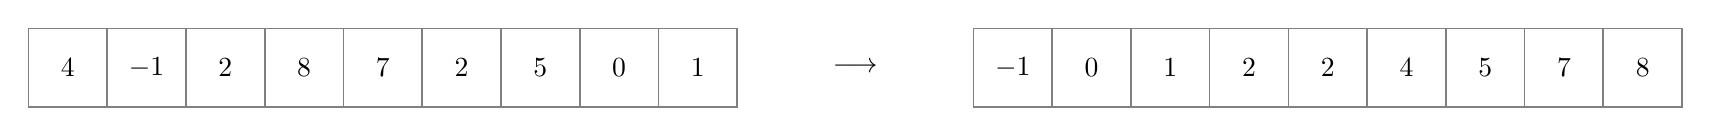
\begin{tikzpicture}[xshift=0.15\textwidth
    , cell/.style = {rectangle,draw=gray,semithick,minimum size=1cm,outer sep = 0mm}
]
\foreach \i [count=\j from 0] in {4, -1, 2, 8, 7, 2, 5, 0, 1}
    \node[cell] at (\j, 0) {$\i$};
\node at (10, 0) {$\longrightarrow$};
\foreach \i [count=\j from 0] in {-1, 0, 1, 2, 2, 4, 5, 7, 8}
    \node[cell] at (\j + 12, 0) {$\i$};
\end{tikzpicture}
}

\vfill
適切な中間目標を設定せよ

\vfill
N/2個のソート問題ふたつに帰着させる。

\begin{itemize}%\itemsep8pt
\item 他方のどの要素よりも小さい要素だけからなる配列
\item 他方のどの要素よりも大きい要素だけからなる配列
\end{itemize}
それぞれを整列、順につなげば全体が整列

\vfill
1ステップごとに範囲が半分の副問題を2つ生成
\end{frame}

\begin{frame}[fragile]{クイックソートRust版下請け関数}{}
\begin{codeof}{language=Rust}{配列を二つに分割(または長さ$N$の配列の並べ替え)}
/// v[beg..end]で最後の要素v[end - 1]以下の要素を[0..i]に移動
/// 注意:[b..e]はeを含まない(bは下限、eは上界)
fn partition<T: Ord>(v: &mut [T], beg: usize, end: usize) -> usize {
    let mut i = beg;
    for j in beg..end {
        if v[j] <= v[end - 1] {
            v.swap(i, j);
            i += 1;
        }
    }
    i
}
\end{codeof}
\end{frame}

\begin{frame}[fragile]{クイックソートRust版}{}
\begin{codeof}{language=Rust}{quick sort}
fn sort<T: Ord>(v: &mut [T], beg: usize, end: usize) {
    if beg + 1 >= end { return; }
    let p = partition(v, beg, end);
    sort(v, beg, p);
    sort(v, p, end);
}

pub fn qsort<T: Ord>(v: &mut [T]) {
    sort(v, 0, v.len());
}
\end{codeof}

\vfill
{\fontsize{9}{9}\selectfont
つないでない。コピーを作らず、その場で並べ替えているので、できたものを移動させる必要がない(in-place search)。
}
\end{frame}

\begin{frame}[fragile]{クイックソートの計算量評価}{最悪計算量、最良計算量、平均計算量}
\begin{columns}[T]
\begin{column}{0.5\textwidth}
\begin{codeof}{language=Rust}{再帰版lsearch}
fn qsort(長さ\@N@)
  長さ\@N@の2分割、または長さ\@N@の並べ替え;
  qsort(長さ\@N/2@);
  qsort(長さ\@N/2@);
\end{codeof}
\end{column}
\begin{column}{0.5\textwidth}
\begin{align*}
T(n) = & ? + T(n/2) + T(n/2) \\
     = & n + 2T(n/2) \\
     = & n \times \log(n) \\
T(N) = & O(N\log(N))
\end{align*}
\end{column}
\end{columns}

\vfill

\begin{columns}[T]
\begin{column}{0.5\textwidth}
木の深さごとに計算量を小計
{
\fontsize{9}{10}\selectfont
\begin{tabular}[h]{| r | r | r |}
\CH 深さ & 作業内容 & 個数 \\
\CL $1$ & N個の並べ替え & $1$ \\
\CL $2$ & $N/2$個の並べ替え & $2$ \\
\CL $3$ & $N/4$個の並べ替え & $4$ \\
\CL $\log_2(N)$ & $1$個の並べ替え & $N$ \\
\end{tabular}
}
\end{column}

\begin{column}{0.5\textwidth}
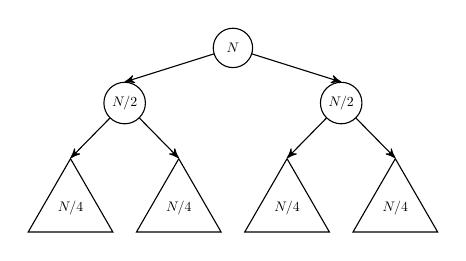
\begin{tikzpicture}[->,>=stealth',level/.style={sibling distance = 5.5cm/#1, level distance = 1.4cm},scale=0.5, transform shape]
\node [treenode] {$N$}
    child[child anchor=north] { node[treenode] {$N/2$}
        child[child anchor=north] { node [subtree] {$N/4$} }
        child[child anchor=north] { node [subtree] {$N/4$} }
    }
    child[child anchor=north] { node[treenode] {$N/2$}
        child[child anchor=north] { node [subtree] {$N/4$} }
        child[child anchor=north] { node [subtree] {$N/4$} }
    }
    ;
\end{tikzpicture}
\end{column}
\end{columns}

\end{frame}

\section{summary}		%%%%%%%%
\subsection{}

\begin{frame}[fragile]{ソートアルゴリズムの比較}{}

{%\fontsize{9}{10}\selectfont
\begin{tabular}[h]{|l|r|r|r|}
\CH アルゴリズム & 時間計算量 & 空間-- & 安定 \\
\CL バブルソート & $O(N^2)$ & $O(1)$ & \checkmark\\
\CL クイックソート & $O(N\log(N))$ & $O(\log(N))$ & \\
\CL ヒープソート & $O(N\log(N))$ & $O(\log(N))$ & \checkmark \\
\CL マージソート & $O(N\log(N))$ & $O(\log(N))$ & \checkmark \\
\end{tabular}
}

\vfill
今回話さなかったこと:2分割できるとは限らないので最悪の場合ではない
\begin{itemize}%\itemsep8pt
\item 要素数が極めて少ない時はバブルソートを使う
\item スタックの消費を嫌って途中からヒープソート
\end{itemize}

\vfill
ヒープソート:データ構造ヒープにデータを登録($O(\log(N))$)、ヒープから取り出し($O(\log(N))$)
\end{frame}

\begin{frame}[fragile]{マージソート}{}
データを二分。再帰的に処理して整列する、それぞれストリームとみなして一つに合成、マージ、整流、zip。

\begin{codeof}{language=Rust}{二つのストリームを第3のストリームにマージする}
fn merge(a: mut stream, b: mut stream, c: stearm) {
    while a.is_empty() && b.is_empty() {
        if aの先頭 < bの先頭 {
          c.push(a.pop());
          if aが空になった { c.append(b); return; }
        } else {
          c.push(b.pop());
          if bが空になった { c.append(a); return; }
        }
    }
}
\end{codeof}
この処理は$O(N)$。全体として$T(n)= T(n/2) + T(n/2) + n$
\end{frame}

\begin{frame}[fragile]{ここまでの振り返り}{アルゴリズム=自明または「前処理$\to$相似問題$\to$後処理」}

{
%\fontsize{9}{10}\selectfont
\begin{tabular}[h]{r l}
\CL 1つを処理、残りを再帰  & $T(n) = 1 + T(n-1) + 0$ \\
\CL 1つを処理、残りを再帰  & $T(n) = 1 + T(n/2) + 0$ \\
\CL 1つを処理、残りを再帰  & $T(n) = n + T(n-1) + 0$ \\
\CL 再帰の準備、再帰、再帰 & $T(n) = n + T(n/2) + T(n/2) + 0$ \\
\CL 再帰、再帰、結果の合成 & $T(n) = 0 + T(n/2) + T(n/2) + n$ \\
\end{tabular}
}

\vfill
これまでの全ての問題において、
\begin{itemize}%\itemsep8pt
\item 中間目標の設定・理解が、問題を解けることに
\item 再帰関数を定義できることが、プログラムを作れることに
\end{itemize}

対応する。
\end{frame}

\begin{frame}[fragile]{}{}
{
\fontsize{14}{14}\selectfont
中学数学の「式を立てる」と同様の「アルゴリズムを立てる」スキルが必要。その上で立てたものを解くスキルが必要。
}
\vfill
\begin{tcolorbox}[colframe=white,colback=black!2!white]
\fontsize{8}{8}\selectfont
\begin{quotation}
「プログラミング的思考」は、文部科学省によると「自分が意図する一連の活動を実現するために、どのような動きの組合せが必要であり、一つ一つの動きに対応した記号を、どのように組み合わせたらいいのか、記号の組合せをどのように改善していけば、 より意図した活動に近づくのか、といったことを論理的に考えていく力」と定義されています。
\end{quotation}
\end{tcolorbox}

\vfill
\begin{center}
\pgfimage[width=0.85\pagewidth]{tekishikou.png}
\end{center}

\begin{tcolorbox}[colframe=white,colback=black!2!white]
\fontsize{6}{6}\selectfont
\begin{quotation}
そして、「すでにコンピューターを使ったプログラミングをやっているよ」という方もぜひ、この番組をご覧ください。プログラミング的思考を育むことで、プログラミングがより上手になるのはもちろん、プログラミング以外の普遍的なシーンでも、その考え方を役立てることができます。
\end{quotation}
\end{tcolorbox}
\end{frame}
\end{document}
